%==============================================================================
% Sjabloon poster bachproef
%==============================================================================
% Gebaseerd op document class `a0poster' door Gerlinde Kettl en Matthias Weiser
% Aangepast voor gebruik aan HOGENT door Jens Buysse en Bert Van Vreckem

\documentclass[a0,portrait]{hogent-poster}

% Info over de opleiding
\course{Bachelorproef}
\studyprogramme{toegepaste informatica}
\academicyear{2025-2026}
\institution{Hogeschool Gent, Valentin Vaerwyckweg 1, 9000 Gent}

% Info over de bachelorproef
\title{LLM's als Assistent-Evaluatoren: 91,1\% Nauwkeurigheid bij Studentenprojecten}
\subtitle{De bruikbaarheid en betrouwbaarheid van LLM-gegenereerde feedback binnen webontwikkeling}
\author{Milan Dhondt}
\email{milan.dhondt@student.hogent.be}
\supervisor{Mevr. V. Depestele}
\cosupervisor{Dhr. T. Aelbrecht}

\usepackage{pgfplots}
\pgfplotsset{compat=1.17}
\begin{document}

\maketitle

\begin{multicols}{2}

\section{Introductie}

Binnen het programmeeronderwijs aan HOGENT (\textit{Front-End Web Development} en \textit{Web Services}) leggen lectoren een enorm repetitief en tijdrovend traject af om studentenprojecten te evalueren. Ze toetsen handmatig tientallen afzonderlijke criteria af per project. Daardoor blijft er structureel minder tijd over om diepgaande kwalitatieve feedback te schrijven, iets wat een student nochtans vaak nodig heeft. Verder zijn repetitieve evaluaties vaak ook oorzaak van inconsistenties.

In deze bachelorproef wordt onderzocht hoe, en in welke mate, Large Language Models (LLM's) ondersteunend kunnen worden ingezet bij deze evaluaties. We richten ons concreet op de bruikbaarheid en betrouwbaarheid van LLM-gegenereerde feedback.

\section{Materialen en Methode}

Dit onderzoek steunde op vijf fases:
\begin{enumerate}
    \item \textbf{Probleemdomeinanalyse}: Interviews met de lectoren om de knelpunten en ervaringen in kaart te brengen.
    \item \textbf{Literatuurstudie}: Onderzoek naar autograding, context limitaties van LLM's, en agentische frameworks.
    \item \textbf{Ontwikkeling PoC}: Via \textbf{Mastra AI} en een E2B cloud-gehoste sandbox werd een veilige pipeline ontwikkeld, aangestuurd door \texttt{qwen3-coder:480b-cloud}.
    \item \textbf{Experiment (Validatie)}: Evaluatie van 8 reeds gequoteerde studentenprojecten.
    \item \textbf{Synthese}: Kwalitatieve en kwantitatieve analyse.
\end{enumerate}

\section{Resultaten}

Uit de analyse van de acht vergeleken projecten kwamen duidelijke patronen naar voor:

\begin{itemize}
    \item \textbf{Hoge accuraatheid ontvankelijkheidscriteria:} Voor ontvankelijkheidscriteria kwam het AI-oordeel in \textbf{91,1\%} van de gevallen geheel overeen met dat van de lectoren.
    \item \textbf{De evaluatiecriteria:} Voor de evaluatiecriteria werkten we met een vergelijkende rubric, gebaseerd op het voorbeeldproject. Hierbij kon een studentenproject op de evaluatiecriteria beter, slechter of gelijkaardig aan het voorbeeldproject scoren.
    \item \textbf{Nauwkeurige referentiëring:} De feedback van het LLM was constructief en kon consistent verwijzen naar specifieke bestanden en lijnen in de base van het studentenproject.
\end{itemize}

\section{Aanwezigheid in Ontvankelijkheid}

De kwantitatieve analyse bevestigde dat de AI voornamelijk op de ontvankelijkheidscriteria een hele hoge graad van consistentie bereikt. In 91 procent van de gevallen kwam het oordeel van het LLM overeen met dat van de lectoren.

\begin{center}
    \captionsetup{type=figure}
    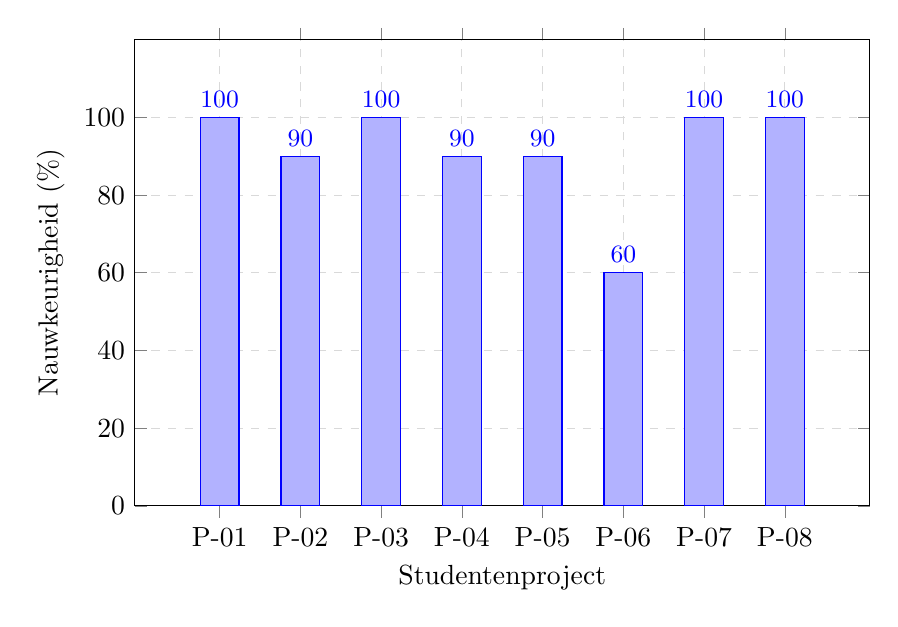
\begin{tikzpicture}
        \begin{axis}[
            ybar,
            width=0.9\linewidth,
            height=7.5cm,
            ylabel={Nauwkeurigheid (\%)},
            symbolic x coords={P-01,P-02,P-03,P-04,P-05,P-06,P-07,P-08},
            xtick=data,
            xlabel={Studentenproject},
            ymin=0, ymax=120,
            ytick={0,20,40,60,80,100},
            bar width=14pt,
            nodes near coords,
            nodes near coords align={vertical},
            every node near coord/.append style={font=\small\bfseries},
            enlarge x limits=0.15,
            grid=major,
            grid style={dashed,gray!30},
            fill=cyan,
            ]
            \addplot coordinates {
                (P-01, 100) (P-02, 90) (P-03, 100) (P-04, 90)
                (P-05, 90) (P-06, 60) (P-07, 100) (P-08, 100)
            };
        \end{axis}
    \end{tikzpicture}
  \captionof{figure}{Vergeleken nauwkeurigheid van de AI-ontvankelijkheidsbeoordeling t.o.v. docenten per project.}
\end{center}

\section{Discussie \& Besluit}
De inzet van LLM-gebaseerde evaluatietools binnen het programmeeronderwijs is zinvol en tijdbesparend. De \textbf{meerwaarde} van dit onderzoek ligt in het aantonen dat een LLM niet enkel code kan schrijven, maar ook autonoom en betrouwbaar (\textit{91,1\% accuraatheid}) ontvankelijkheidscriteria kan detecteren. Hoewel menselijke controle vereist blijft, kan deze AI-oplossing het evaluatieproces aanzienlijk verlichten. Bovendien levert de uiterst gedetailleerde feedback een sterke didactische meerwaarde voor de student.

\section{Toekomstig onderzoek}
In toekomstig onderzoek kan de flow nog uitgebreid worden om de lectoren te ondersteunen bij het voorbereiden van de mondelinge evaluaties. Dit zou gedaan kunnen worden door vreemde implementaties of andere bijzonderheden in het project te laten highlighten, en hier eventueel al vragen over te genereren, zodat de lectoren hierop kunnen in gaan tijdens de mondelinge evaluatie. Verder zou de consistentie van de PoC verder verhoogd kunnen worden door de projectstructuur over alle projecten gelijk te proberen trekken, of om de studenten hun projectstructuur zeer duidelijk te laten documenteren.

\section{Referenties}
De bachelorproef en Poc zijn te vinden op\newline \texttt{https://github.com/milandhondt/Bachelorproef-25-26-MD}.

\end{multicols}
\end{document}